% !TEX encoding = UTF-8 Unicode
% !TEX spellcheck = en-US


% This is the root file of your thesis: thesis.tex
% A line starting with % is a comment. In some cases, I have included a command preceded by a %. You may activate the command by removing the %.

%%===================================
\documentclass[12pt]{report}
\usepackage{ramsstyle}

%%===================================
%Write the various parts of your thesis as separate files and include them into the main file by the command \include{name of included file}. When you compile the LaTeX file, you may choose which subfiles to include by the command

%\includeonly{chapter01,chapter02}

%%===================================
\begin{document}
% !TEX encoding = UTF-8 Unicode
%!TEX root = thesis.tex
% !TEX spellcheck = en-US

%This is the Titlepage
%%=========================================
\thispagestyle{empty}
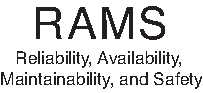
\includegraphics[scale=1.1]{fig/rams}
\mbox{}\\[6pc]
\begin{center}
\Huge{This is the Title of my Thesis}\\[2pc]

\Large{Your Name}\\[1pc]
\large{August 2014}\\[2pc]

PROJECT / MASTER THESIS\\
Department of Production and Quality Engineering\\
Norwegian University of Science and Technology
\end{center}
\vfill

\noindent Supervisor 1: Professor Ask Burlefot

\noindent Supervisor 2: Professor Fingal Olsson

 % This is the titlepage
\setcounter{page}{0}
\pagenumbering{roman}
% !TEX encoding = UTF-8 Unicode
%!TEX root = thesis.tex
% !TEX spellcheck = en-US
%%=========================================
\addcontentsline{toc}{section}{Preface}
\section*{Preface}
Here, you give a brief introduction to your work. What it is (e.g., a Master's thesis in RAMS at NTNU as part of the study program xxx and\ldots), when it was carried out (e.g., during the autumn semester of 2021). If the project has been carried out for a company, you should mention this and also describe the cooperation with the company. You may also describe how the idea to the project was brought up.

You should also specify the assumed background of the readers of this report (who are you writing for).\\[2cm]

\begin{center}
Trondheim, 2012-12-16\\[1pc]
(Your signature)\\[1pc]
Ola Nordmann
\end{center}
%% !TEX encoding = UTF-8 Unicode
%!TEX root = thesis.tex
% !TEX spellcheck = en-US
%%=========================================
\addcontentsline{toc}{section}{Acknowledgment}
\section*{Acknowledgment}
I would like to thank the following persons for their great help during \ldots

If the project has been carried out in cooperation with an external partner (e.g., a company), you should acknowledge the contribution and give thanks to the involved persons.

You should also acknowledge the contributions made by your supervisor(s).

\begin{flushright}
O.N.\\[1pc]
(Your initials)
\end{flushright}
% !TEX encoding = UTF-8 Unicode
%!TEX root = thesis.tex
% !TEX spellcheck = en-US
%%=========================================
\addcontentsline{toc}{section}{Summary and Conclusions}
\section*{Summary and Conclusions}
Here you give a summary of your your work and your results. This is like a management summary and should be written in a clear and easy language, without many difficult terms and without abbreviations. Everything you present here must be treated in more detail in the main report. You should not give any references to the report in the summary -- just explain what you have done and what you have found out. The Summary and Conclusions should be no more than two pages.

You may assume that you have got three minutes to present to the Rector of NTNU  what you have done and what you have found out as part of your thesis. (He is an intelligent person, but does not know much about your field of expertise.)
\tableofcontents
\setcounter{page}{0}
\pagenumbering{arabic}
%% !TEX encoding = UTF-8 Unicode
%!TEX root = thesis.tex
% !TEX spellcheck = en-US
%%=========================================
\chapter{Introduction}
\textcolor{red}{REF TO {\tt{R}} \cite{r}.}\\
\\
\\
The first chapter of a well-structured thesis is always an introduction, setting the scene with background, problem description, objectives, limitations, and then looking ahead to summarize what is in the rest of the report. This is the part that readers look at first---\emph{so make sure it hooks them!}

%%=========================================
\section{Background}
In this section, you should present the problem that you are going to investigate or analyze; why this problem is of interest; what has, so far, been done to solve the problem, and which parts of the problem that remain.

{\color{red}Below, I have set up some headings (subsection titles) without a number. These are included to help you remember to cover the related issues. The headings should be removed in your final print.}
%%=========================================
\subsection*{Problem Formulation}
You should define your problem in a clear an unambiguous (clear only one meaning) way and explain why this is a problem, why it is of interest---and to whom. It is also important to delimit the problem area.
%%=========================================
\subsection*{Literature Survey}
You should here present the main books and articles that treat problems that are similar to what  you are studying. If you,  later in your thesis, describe the ``state of the art'' -- with a detailed literature survey, you may just give a very brief survey here (approx. a quarter of a page). If this is the only literature survey, you need to go into more details. An objective of the literature survey is to show the reader that you are familiar with the main literature within your field of research -- so that you do not ``reinvent the wheel.''


References to literature can be given in two different ways:
\begin{itemize}
\item As an \emph{explicit} reference: It is shown by \citet{lundteigen08} and partly also by \citet{rausand14}  that \ldots.
\item As an \emph{implicit} reference: It is shown \citep[e.g., see][Chap. 4]{rausand04} that \ldots.
\end{itemize}
In the example above, we have used ``author-year'' references, which is the preferred format. 
\begin{remark}
Following agreement with your supervisor, you may also refer by numbers, for example,  [1]. To do this, open the file \texttt{ramsstyle.sty} and  comment out (by \%) the command \texttt{$\backslash$usepackage\{natbib\}} and un-comment the corresponding command \texttt{$\backslash$usepackage[numbers]\{natbib\}}.\footnote{Notice the strange way we have to write the ``backslash'' in the text. This is because the ``backslash'' is a command in \LaTeX.}
\end{remark}
 You may include a link to the Internet in the text or in a footnote by using a command like: \url{http://www.ntnu.edu/ross}. 

When you refer to the scientific literature, you should always write in \emph{present} tense. Example: \citet{rausand04} show that \ldots.

\begin{remark}
Hyperlinks are included by the command \texttt{$\backslash$usepackage\{hyperref}\} in \texttt{ramsstyle.sty}. If you feel that the hyperlinks are disturbing when you enter the text, or want to avoid the hyperlinks in printed text, you may either comment out or edit this command in \texttt{ramsstyle.sty}.
\end{remark}
%%=========================================
\subsection*{What Remains to be Done?}
After you have defined and delimited your problem -- and presented the relevant results found in the literature within this field, you should sum up which parts of the problem that remain to be solved.
%%=========================================
\section{Objectives}
The main objectives of this Master's project are
\begin{enumerate}
\item This is the first objective
\item This is the second objective
\item This is the third objective
\item More objectives
\end{enumerate}

The objectives shall be written as \emph{fundamental objectives} telling what to do and not \emph{means objectives} telling how to do it.

All objectives shall be stated such that we, after having read the thesis, can see whether or not you have met the objective. ``To become familiar with \ldots'' is therefore not a suitable objective.

%%=========================================
\section{Limitations}
In this section you describe the limitations of your study. These may be related to the study object (physical limitations, operational limitations), to the environmental and operational conditions, to the thoroughness of the analysis, and so on. (Kris computational limitations!!)
%%=========================================
\section{Approach}
Here you should describe the (scientific) approach that you will use to solve the problem and meet your objectives. You should specify the approach for each objective.

If there are any ethical problems related to your approach, these should be highlighted and discussed.
%%=========================================
\section{Structure of the Report}
The rest of the report is organized as follows. Chapter 2 gives an introduction to \ldots

\begin{remark}
Notice that chapter and section headings shall be written in lowercase, but that all main words should start with a capital letter.
\end{remark}


The report should be no longer than \underline{60 pages} in this format (+ the CV).
\chapter[Theory]{Theory}
This chapter gives an introduction of/to the theory behind this thesis/paper. Some of the following sections only give a brief description of the theory whit sources for more in depth explanation. The main focus of this chapter is describing the theory behind the Markov chain Mote Carlo method for solving extreme value problem developed for this paper. 
\section{Extreme value theory}
peak over threshold..
\section{Average Condition Exceedance Rate}
blabla

\section{Bayesian Inference}
\label{ch:BayesianInference}

\section{Markov Chain Monte Carlo Method}
Markov Chain Monte Carlo (MCMC) is a powerful iterative method used to sample from probability distributions, which analytically or through other simulation methods, could be difficult and impracticable to sample from. The algorithm is constructed by converging the desired probability distribution to an irreducible and aperiodic Markov Chain with limiting distribution equal the target distribution. Independent of starting position the Markov Chain will then converge towards the desired probability distribution in the limit as the numbers of iterations goes to infinity. The first numbers of realizations from the Markov Chain until converging is called the burn-in period, and is discarded for further analyses. The remaining realizations, approximately follows the desired probability distribution, where the accuracy increase as the numbers of realizations increase. Monte Carlo method can then be used to calculate the quantity of interest like mean, expected value, future prediction, credible interval etc.

\subsection{Gibbs Sampling}
In situations where it is difficult to sample from the joint distribution, but applicable from the conditional distribution, Gibbs sampler is preferable. The principle of Gibbs sampling is to construct the Markov Chain, by repeatedly sample each parameter with the rest of the parameters as the condition. The Gibbs sampler start with an initial guess $\boldsymbol{X}^{0}=[X_1^0,\cdots, X_n^0]$ for the parameters, then iteratively update each as follows
\begin{align}
\label{eq:gibbs}
\begin{split}
    X_1^{t+1}& \sim f(X_1|X_2^{t},\cdots,X_n^{t}),\\
    X_2^{t+1}& \sim f(X_2|X_1^{t+1},X_3^{t},\cdots,X_n^{t}),\\
    \vdots \\
    X_n^{t+1}& \sim f(X_n|X_1^{t+1},\cdots,X_{n-1}^{t+1}).
\end{split}
\end{align}
where....
The iterative process is repeated until enough realizations are generated for sufficient accuracy.\\
REFFF!!

\subsection{Metropolis–Hastings Algorithm}
Metropolis–Hastings algorithm is another method for constructing a suitable Markov Chain. The algorithm is preferable for situations where a proportional distribution is simple to evaluate, while the target probability distribution is difficult. Bayesian inference (see chapter \ref{ch:BayesianInference}), often result in a distribution where the normalizing constant cannot analytically be calculated. While possible numerically, the normalizing constant often becomes computationally hard, which make it impracticable for iterative simulations. Using Metropolis–Hastings algorithm on a proportional distribution whiteout normalizing constant, results in samples from the target distributions. The Metropolis–Hastings algorithm start with an initial guess for the parameters. For each iteration a new parameters $\boldsymbol{X} \mbox{*}$ are suggested from a proposal distribution $g(\boldsymbol{X} \mbox{*}|\boldsymbol{X}^t)$, given the last accepted parameter $\boldsymbol{X}^t$. The new parameter is then evaluated against the last accepted by
\begin{equation}
R(\boldsymbol{X} \mbox{*},\boldsymbol{X}^{t})=\frac{f(\boldsymbol{X} \mbox{*})g(\boldsymbol{X}^{t}|\boldsymbol{X} \mbox{*})}{f(\boldsymbol{X}^{t})g(\boldsymbol{X} \mbox{*}|\boldsymbol{X}^{t})}
\end{equation}
where $f(x)$ is the target distribution, or a distribution proportional to the target distribution. The parameter $\boldsymbol{X}^{t+1}$ takes value $\boldsymbol{X}\mbox{*}$ with probability $\min\{1,R(\boldsymbol{X} \mbox{*},\boldsymbol{X}^{t})\}$, if rejected, $\boldsymbol{X}^{t+1}=\boldsymbol{X}^t$ instead.

The Metropolis–Hastings algorithm could in situations be necessary for some of the steps in the Gibbs sampler, equation \eqref{eq:gibbs}. A combination of Metropolis-Hastings algorithm and Gibbs sampler is referred to as a Hybrid Gibbs sampler.  

REFFF!!\\
%
%
hybrid as in \eqref{eq:gibbs}.
REFFF!!\\
\subsection{Adaptive Metropolis–Hastings Algorithm}


\subsection{Effective Sample Size}
The realizations of the simulated Markov Chain will often be correlated, and dependent on the future and past iterations. The correlation implies that the information hold by the realizations is actually less than the numbers of realizations. The effective sample size gives a method of calculating the theoretical size of an equally informative independent and identical distributed, realization set. The effective sample size is estimated as
\begin{equation}
L_{eff}=\frac{L}{1+2\sum_{k=1}^{K}\hat{\rho}(k)},
\end{equation}
Where $L$ is the realizations of the sample size, $\hat{\rho}(k)$ is the estimated $k$ step autocorrelation between realizations and $K$ is chosen as the first $k$ where $\hat{\rho}(k)<0.1$ ref(BOK COMP STAT).

\section{Applying Markov Chain Monte Carlo to Peak Over Threshold}
The left side of equation \ref{eq:POT} can be written as %what is x,u...? described in eq:POT!
\begin{equation}
\Pr(X>x|X>u)=\frac{\Pr(X>x,X>u)}{\Pr(X>u)}, 
\end{equation}
where the nominator $\Pr(X>x,X>u)=\Pr(X>x)$, since the conditional distribution require $x>u$. Reorganizing \ref{eq:POT} gives
\begin{equation}
\Pr(X>x)=\Pr(X>u)\cdot \left[1+\xi \left( \frac{x-u}{\sigma}\right)\right]^{-\frac{1}{\xi}}.
\label{eq:ConProbGev}
\end{equation}
%
%
%
%
%
Usefull to have as much knowledge as possible abouth the target distribution as possible=> better simmulation ish 23\% acceptance.\\
Prior distribution hard to choose.... future improvements!!
%
irreducible if its state space is a single communicating class; in other words, if it is possible to get to any state from any state. check.\\
aperiodic if there exists n such that for all n'>n $\Pr(X_{n'}=i|X_0=i)>0$ 


%p(X>x|X>u)=\frac{p(X>x,X>u)}{p(X>u}=\frac{p(X>x)}{p(X>u)}$ since the condition require x>u.

\subsection{Multivariate Random Normal Generator}
lkajsd yous tla blaa 
\section{Value at Risk}
mer bla bla
\section{ARCH/GARCH}%????
is this needed????
\chapter[Data]{Data}
\label{ch:data}
hei
\section{Synthetic Data}
blabla
\subsection{Pareto}
sim sim
\subsection{Commodity Generated Data}
sam sam
\section{Commodity Data}
\label{ch:comdata}
Adjusted for the roll-over returns. (simply done by deleting the return at the roll-over date).(roll-over, en kontrakt til neste eks sommer til hoest, kan gi ekstreme returns som gir  forvrengende resultater).
blabla
%% !TEX encoding = UTF-8 Unicode
%!TEX root = thesis.tex
% !TEX spellcheck = en-US
%%=========================================
\chapter[Equations, etc]{Equations, Figures, and Tables}
The content of Chapter 2 will vary with the topic of your thesis. This chapter only gives guidance to some technical aspects of \LaTeX.
 
\begin{remark}
If you want a shorter chapter or section title to appear in the Table of Contents and in the headings of the chapter, you just include the short title in square brackets before the title of the chapter/section. Example: \begin{verbatim}\section[Short Title]{Long Title}\end{verbatim}.
\end{remark}

%%=========================================
\section{Simple Equations}
Mathematical symbols and equations can written in the text as $\lambda$, $F(t)$, or even $F(t)=\int_0^t \exp(-\lambda x)\,dx$, or as displayed equations
\begin{equation}
F(t)=\int_0^t \exp(-\lambda x)\,dx
\label{eq1}
\end{equation}


The displayed equations are automatically given equation numbers -- here (\ref{eq1}) since this is the first equation in Chapter 2. Note that you can refer to the equation by referring to the ``label'' you specified as part of the equation environment.

You can also include equations without numbers:
\begin{equation*}
F(t)=\sum_{i=1}^n \binom{n}{i}\sin(i\cdot t)
\end{equation*}

%%=========================================
\subsection*{More Advanced Formulas}
Long formulas that cannot fit into a single line can be written by using the environment \texttt{align} as
\begin{align}
F(t)&= \sum_{i=1}^n \sin(t^{n-1}) - \sum_{i=1}^n \binom{n}{i}\sin(i\cdot t) \\
      & + \int_0^\infty n^{-x} e^{-\lambda x^t}\,dt
\end{align}

In some cases, you need to write ordinary letters inside the equations. You should then use the commands 
\begin{verbatim}
\textrm  and/or \mathrm
\end{verbatim}
The first command returns the normal text font and will be scaled automatically, while the second command will be scaled according to the use.
\begin{equation*}
\textrm{MTTF}= \int_0^\infty R_\mathrm{avg}(t)\,dt
\end{equation*}



Please consult the \LaTeX\ documentation for further details about mathematics in \LaTeX.
%%=========================================
\section*{Definitions}
If you want to include a definition of a term/concept in the text, I have made the following macro (see in \texttt{ramsstyle.sty}):
\begin{defin}
\textbf{Reliability}: The ability of an item to perform a required function under stated environmental and operational conditions and for a stated period of time.\newline
\end{defin}
When text is following directly after the definition, it may sometimes be necessary to end the definition text by the command
\begin{verbatim}
\newline
\end{verbatim}
I have not included this in the definition of the \texttt{defin} environment to avoid too much space when there is not a text-block following the definition.
%%=========================================
\section{Including Figures}
If you use pdf\LaTeX\ (as recommended), all the figures must be in pdf, png, or jpg format. We recommend you to use the pdf format.  Please place the figure files in the directory \textbf{fig}. Figures are included by the command shown for Figure~\ref{fig1}. Please notice the ``path'' to the figure file written by a \emph{forward} slash (/). You should not include the format of the figure file (pdg, png, or jpg) -- just write the ``name'' of the figure. 
\begin{figure}
\centering

\includegraphics[scale=0.6,angle=15]{fig/NTNU}
\caption{This is the logo of NTNU (rotated 15 degrees).}
\label{fig1}
\end{figure}

Each figure should include a unique \emph{label} as shown in the command for Figure~\ref{fig1}. You can then refer to the figure by the \emph{ref} command.
Notice that you can scale the size of the figure by the option \texttt{scale=k}. You may also define a specific width or height of the figure by replacing the \texttt{scale} options by \texttt{width=k} or \texttt{height=k}. The factor \texttt{k} can here be specified in mm, cm, pc, and many other length measures. You may also give \texttt{k} as a fraction of the width of the text or of the height of the text, for example, \texttt{width=0.45$\backslash$textwidth}. If you later change the margins of the text, the figure width will change accordingly. As illustrated in Figure~\ref{fig1}, you may also rotate the figure -- and also do many other things (please check the documentation of the package \texttt{graphicx} -- it is available on your computer, or you may find it on the Internet).

In \LaTeX\ all figures are floating objects and will normally be placed at the top of a page. This is the standard option in all scientific reports. If you insist on placing the figure exactly where you declare the figure, you may include the command \texttt{[h]} (here) immediately after $\backslash$\texttt{begin\{figure\}}. If you will force the figure to be located either at the top or bottom of the page, you may alternatively use  \texttt{[t]} or \texttt{[b]}. For more options, check the documentation.

Large figures may be included as a \emph{sidewaysfigure} as shown in Figure~\ref{fig2}:\footnote{You can use a similar command for large tables.}
\begin{sidewaysfigure}
\centering

\includegraphics[scale=1.8]{fig/NTNU}
\caption{This is the logo of NTNU.}
\label{fig2}
\end{sidewaysfigure}

%%=========================================
\section{Including Tables}
\LaTeX\ has a lot of different options to include tables. Only one of them is illustrated here.

\begin{table}
	\centering\small
	\caption{The degree of newness of technology.}
	\label{tab1}
		\begin{tabular*}{\textwidth}{@{\extracolsep{\fill}}lccc}
			\toprule
			  &\multicolumn{3}{c}{Level of technology maturity}\\
  \cmidrule{2-4}
			Experience with the		   &  & Limited field history or not & New or \\
              operating  condition  & Proven &  used by company/user & unproven \\
        
			\midrule
			  Previous experience & 1 & 2 & 3 \\
		          No experience by company/user & 2 & 3 & 4 \\
		          No industry experience & 3 & 4 & 4 \\
			\bottomrule
		\end{tabular*}
\end{table}

\begin{remark}
Notice that figure captions (Figure text) shall be located \emph{below} the figure -- and that the caption of tables shall be \emph{above} the table. This is done by placing the $\backslash$\texttt{caption} command beneath the command $\backslash$\texttt{includegraphics} for figures, and above the command $\backslash$\texttt{begin\{tabular*\}} for tables.
\end{remark}
%%=========================================
\section{Copying Figures and Tables}
In some cases, it may be relevant to include figures and tables from from other publications in your report. This can be a direct copy or that you retype the table or redraw the figure. In both cases, you should include a reference to the source in the figure or table caption. The caption might then be written as: \textsl{Figure/Table xx: The caption text is coming here \citep{rausand04}.}

In other cases, you get the idea from a figure or table in a publication, but modify the figure/table to fit your purpose. If the change is significant, your caption should have the following format: \textsl{Figure/Table xx: The caption text is coming here \citep[adapted from][]{rausand04}.}

%%=========================================
\section{References to Figures and Tables}
Remember that all figures and tables shall be referred to and explained/discussed in the text. If a figure/table is not referred to in the text, it shall be deleted from the report.
%%=========================================
\section{A Word About Font-encoding}
When you press a button (or a combination of buttons) on your keyboard, this is represented in your computer according to the \emph{font-encoding} that has been set up. A wide range of font-encodings are available and it may be difficult to choose the ``best'' one. In the template, I have set up a font-encoding called UTF-8 which is a modern and very comprehensive encoding and is expected to be the standard encoding in the future. Before you start using this template, you should open the Preferences ->Editor dialogue in TeXworks (or TeXShop if you use a Mac) and check that encoding UTF-8 has been specified. 

If you use only numbers and letters used in standard English text, it is not very important which encoding you are using, but if you write the Norwegian letters æ, ø, å and accented letters, such as é and ä, you may run into problems if you use different encodings. Please be careful if you cut and paste text from other word-processors or editors into your \LaTeX\ file!

\subsubsection*{Warning}
If you (accidentally) open your file in another editor and this editor is set up with another font-encoding, your non-standard letters will likely come out wrong. If you do this, and detect the error, be sure \emph{not} to save your file in this editor!!

This is not a specific \LaTeX\ problem. You will run into the same problem with all editors and word-processors -- and it is of special importance if you use computers with different platforms (Windows, OSX, Linux).

%%=========================================
\section{Plagiarism}
Plagiarism is defined as ``use, without giving reasonable and appropriate credit to or acknowledging the author or source, of another person's original work, whether such work is made up of code, formulas, ideas, language, research, strategies, writing or other form'', and is a very serious issue in all academic work. You should adhere to the following rules:
\begin{itemize}
\item Give proper references to all the sources you are using as a basis for your work. The references should be give to the original work and not to newer sources that mention the original sources.
\item You may copy paragraphs up to 50 words when you include a proper reference. In doing so, you should place the copied text in inverted commas (i.e., ``Copied text follows \ldots''). Another option is to write the copied text as a quotation, for example:
\begin{quote}
Birnbaum's measure of reliability importance of component $i$ at time $t$ is equal to the probability that the system is in such a state at time $t$ that component $i$ is critical for the system.\newline \mbox{} \hfill \citet{rausand04}
\end{quote}
\end{itemize}




% !TEX encoding = UTF-8 Unicode
%!TEX root = thesis.tex
% !TEX spellcheck = en-US
%%=========================================
\chapter[Summary]{Summary and Recommendations for Further Work}
Better prior MCMC (Improved prior)$=>$ higher effective sample size.\\
GEV instead of POT! (since AR-GARCH $\sim$ i.i.d).\\
Improved ACER program. ACER continious CI so qq-plot is possible (given a 1\% event, where on the extreme prediction confidence level is that)\\
Automatically selecting u for POT MCMC each turn.\\
REMEMBER IN THEORY, WHY ADAPTIVE MCMC!! MAX EFFECTIVE SAMPLE SIZE, AND MORE IMPORTANTLY AUTOMATIC!!!!! MINIMAL HUMA INTERACTION.\\

%%This is the last chapter
%In this final chapter you should sum up what you have done and which results you have got. You should also discuss your findings, and give recommendations for further work.

%%=========================================
\section{Summary and Conclusions}
Here, you present a brief summary of your work and list the main results you have got. You should give comments to each of the objectives in Chapter 1 and state whether or not you have met the objective. If you have not met the objective, you should explain why (e.g., data not available, too difficult).

This section is similar to the Summary and Conclusions in the beginning of your report, but more detailed---referring to the the various sections in the report.

%%=========================================
\section{Discussion}
Here, you may discuss your findings, their strengths and limitations.
%%=========================================
\section{Recommendations for Further Work}
You should give recommendations to possible extensions to your work. The recommendations should be as specific as possible, preferably with an objective and an indication of a possible approach.

The recommendations may be classified as:
\begin{itemize}
\item Short-term
\item Medium-term
\item Long-term
\end{itemize}
% Include more chapters as required.
%%=========================================
\appendix
%% !TEX encoding = UTF-8 Unicode
%!TEX root = thesis.tex
% !TEX spellcheck = en-US
%%=========================================

\chapter{Acronyms}
\begin{description}
\item[FTA] Fault tree analysis
\item[MTTF] Mean time to failure
\item[RAMS] Reliability, availability, maintainability, and safety
\end{description}
% !TEX encoding = UTF-8 Unicode
%!TEX root = thesis.tex
% !TEX spellcheck = en-US
%%=========================================

\chapter{Additional Information}
This is an example of an Appendix. You can write an Appendix in the same way as a chapter, with sections, subsections, and so on.

%%=========================================
\section{Introduction}

%%=========================================
\subsection{R}
\lstset{style=mystyleR}
\begin{lstlisting}[language=R]
#Dette er en melding 
string<-"Heisann du"
a=5
for(i in 1:a){
	print(i)
}
bla
blla
\end{lstlisting}



\subsection{C++}
\lstset{style=mystyleCpp} 
\begin{lstlisting}[language=C++]
#include<stdio.h>
#include<iostream>
// A comment
int main(void)
{
  for(int i=0;i<5;i++){
     cout<<i;
  }
  printf("Hello World\n");
  return 0;
}
\end{lstlisting}
% Include more appendices as required.
%%=========================================
\bibliographystyle{apa}
\addcontentsline{toc}{chapter}{\bibname}
\bibliography{refs}  
%%=========================================
%% !TEX encoding = UTF-8 Unicode
%!TEX root = thesis.tex
% !TEX spellcheck = en-US

%This is the Curriculum Vitae
%%=========================================
\addcontentsline{toc}{chapter}{Curriculum Vitae}
\chapter*{Curriculum Vitae}
\hrule
\begin{minipage}[t]{0.65\linewidth}
\begin{tabular}{ll}
Name: & \textbf{Your Name}\\
Gender: & Female\\
Date of birth: & 1. January 1995\\
Address: & Nordre gate 1, N--7005 Trondheim \\
Home address: & King's road 1, 4590 Vladivostok, Senegal\\
Nationality:    & English \\
Email (1): & your.name@stud.ntnu.no\\
Email (2): & yourname@gmail.com\\
Telephone: & +47 12345678\\
\end{tabular} 
\end{minipage}\hfill
\begin{minipage}[t]{0.25\linewidth}
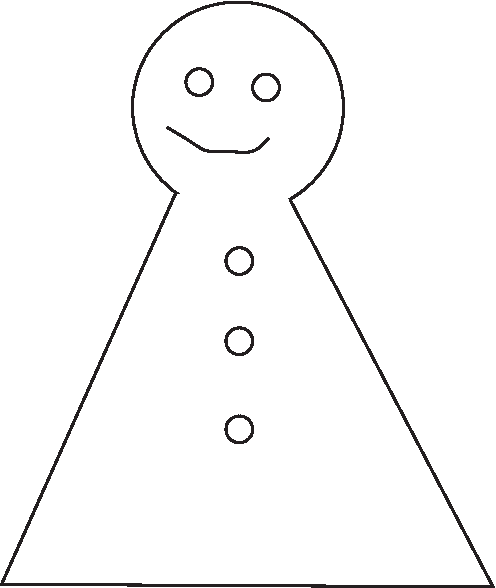
\includegraphics[scale=0.3]{fig/me}\\[1pc] Your picture
\end{minipage}
\hrule

%%=========================================
\section*{Language Skills}
Describe which languages you speak and/or write. Specify your skills in each language.

%%=========================================
\section*{Education}
\begin{itemize}
\item School 1
\item School 2
\item School 3
\end{itemize}

%%=========================================
\section*{Computer Skills}
\begin{itemize}
\item Program 1
\item Program 2
\item Program 3
\end{itemize}

%%=========================================
\section*{Experience}
\begin{itemize}
\item Job 1
\item Job 2
\item Job 3
\end{itemize}

%%=========================================
\section*{Hobbies and Other Activities}         % Your curriculum Vitae     
%%=============================================

\end{document}
